% !TEX root = epifanov_solid_state_physics.tex
%!TEX TS-program = pdflatex
%!TEX encoding = UTF-8 Unicode


\chapter[Thermal Properties of Solids]{Thermal Properties of Solids}\label{chap:4}
% \chaptermark{Bonding. The Internal Structure of Solids}

\section{Normal modes of a lattice}\label{sec:30}

The atoms of a solid take part in thermal vibrations around their equilibrium positions. Because of a strong interaction between them, the nature of those vibrations turns out to be extremely complex and an accurate description of it presents enormous difficulties. Therefore, approximate methods and various simplifications are used to solve this problem.

Instead of describing the individual vibrations of the particles the practice is to consider their collective motion in the crystal, which is a spatially ordered structure. This simplification is based on the fact that powerful bonds immediately transmit the vibrations of one particle to other particles and a collective motion in the form of an elastic wave involving all the particles of the crystal is excited in it. Such collective motion is called the \textit{normal mode of a lattice}. The number of normal modes coincides with the number of degrees of freedom, which is $3N$ if $N$ is the number of particles constituting the crystal.

Figure \ref{fig:4_1}(a) represents a one-dimensional model of a solid---a linear chain of atoms separated by a distance $a$ and able to vibrate in the direction perpendicular to the chain. Such a chain may be regarded as a string. If the ends of the chain are fixed, the fundamental mode corresponding to the lowest frequency $\ab{\omega}{min}$ is represented by the standing wave with a node at each end [\fig{4_1}(b), curve $1$]. The second mode is represented by the standing wave with an additional node in the centre of the chain (curve $2$). The third mode, or third harmonic, is represented by the standing wave with two additional nodes that divide the chain in three equal parts (curve $3$), etc. The length of the shortest wave in such a chain is evidently equal to twice the distance between the atoms of the chain [\fig{4_1}(c)]:
\begin{equation}\label{eq:4_1}
    \ab{\lambda}{min} = 2 a.
\end{equation}

\noindent
The corresponding maximum frequency $\ab{\omega}{max}$ is
\begin{equation}\label{eq:4_2}
    \ab{\lambda}{max} = \frac{2\pi v}{\ab{\lambda}{min}} = \frac{\pi v}{a}
\end{equation}

\noindent
where $v$ is the velocity of wave propagation (of sound) along the chain.

\begin{figure}[t]
	\begin{center}
		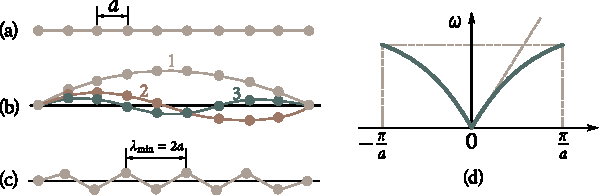
\includegraphics[scale=1.1]{figures/ch_04/fig_4_1.pdf}
		\caption[]{Normal modes of a linear chain made up of identical atoms: (a)---linear chain; (b)---normal modes of the chain; (c)---normal modes of the chain corresponding to shortest wavelength (to highest frequency); (d)---dispersion curves expressing dependence of normal mode frequency on wave vector.}
		\label{fig:4_1}
	\end{center}
	\vspace{-0.7cm}
\end{figure}

This maximum frequency is a parameter of the chain's material and is determined by the interatomic distance and the velocity of wave propagation. Should we set $a=\SI{3.6e-10}{\metre}$ (the lattice parameter of copper) and $v=\SI{3550}{\metre\per\second}$ (the velocity of sound in copper) we would obtain $\ab{\omega}{max}\approx\SI{3e13}{\per\second}$, which corresponds to the frequency of atomic vibrations in a solid.

To describe wave processes one usually uses the wave vector $\vec{q}$ whose direction coincides with that of wave propagation and whose absolute value is
\begin{equation}\label{eq:4_3}
    q = \frac{2\pi}{\lambda}.
\end{equation}

\noindent
It follows from \eqn{4_2} that $2\pi/\lambda=\omega/v$. Therefore\footnote{The phase velocity $v$, which enters \eqref{eq:4_4}, is itself a function of the wave vector $\vec{q}$ and for a linear chain of atoms bonded by elastic forces is expressed by the following relation:
\begin{equation}\label{eq:4_4p}
    v = v_0 \frac{\sin(qa/2)}{(qa/2)} \tag{4.4$'$}
\end{equation}

\noindent
where $v_0$ is the velocity of wave propagation in a continuous string for which $a=0$. It follows from \eqn{4_4p} that for a constant $a$, the velocity $v$ is practically independent of $\vec{q}$ and is approximately $v_0$ only in the range of small $q'$s, where $[\sin(qa/2)]/(qa/2)\ll 1$. In this range $\omega$ increases approximately in proportion to $q$ [\fig{4_1}(d)].
As $q$ increases, the value of $[\sin(qa/2)]/(qa/2)\ll 1$ steadily diminishes and for $q=\pi/a$ tends to $2/\pi$. This causes the dispersion curve $\omega(q)$ to flatten out, so that for $q=\pi/a$ it runs parallel to $q$.},
\begin{equation}\label{eq:4_4}
    q = \frac{\omega}{v} \quad\Rightarrow\quad  \omega = q v.
\end{equation}

Figure \ref{fig:4_1}(d) shows the dependence on wave vector $q$ of the frequency of normal modes in a linear chain made up of atoms of one kind. As $q$ increases from $0$ to $\pi a$, the frequency of the normal modes rises, reaching the maximum value $\ab{\omega}{max}=\pi v/a$ for $q=\pi/a$, that is, for $\lambda=2a$. Curves of this type expressing the dependence of the vibration frequency on the wave vector (the wavelength) are termed \textit{dispersion curves}.

Consider now a chain made up of atoms of two kinds placed in a regular sequence one after another [\fig{4_2}(a)]. Denote the mass of the heavier atoms by $M$ and that of the lighter atoms by $m$. Two types of normal modes can be present in such a chain, as is shown in \fig{4_2}(b,c). The modes in \fig{4_2}(b) are quite identical to the modes of a uniform chain: the phases of the neighbouring atoms are practically the same. Such vibrations are termed \textit{acoustic modes}, since they include the entire spectrum of the acoustic modes of the chain. For them, $\ab{\omega}{ac}=0$ for $q=0$. They play a decisive part in determining the thermal properties of the crystals such as heat capacity, heat conductivity, thermal expansion, etc.

\begin{figure}[t]
	\begin{center}
		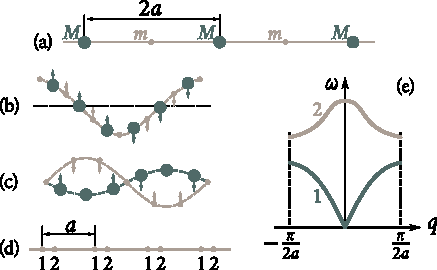
\includegraphics[scale=1.1]{figures/ch_04/fig_4_2.pdf}
		\caption[]{Normal modes of a chain made up of atoms of two kinds: (a)---arrangement of atoms in the chain; (b)---acoustic modes; (c)---optical modes; (d)---dispersion curves for acoustic and optical modes; (e)---linear lattice with a basis in which optical and acoustic modes are present.}
		\label{fig:4_2}
	\end{center}
	\vspace{-0.7cm}
\end{figure}

In case of normal modes shown in \fig{4_2}(c) the phases of the neighbouring vibrating atoms are opposite. Such modes can be treated as the relative vibrations of two interpenetrating sublattices, each made up of atoms of one kind. They are termed \textit{optical modes}, since they play a decisive part in the processes of interaction of light with crystals.

Figure \ref{fig:4_2}(d) shows the dispersion curves for the acoustic ($1$) and optical ($2$) normal modes of a chain made up of atoms of two kinds. In contrast to an acoustic mode, whose frequency rises with the wave vector reaching the maximum value at $\ab{q}{max}=\pi/(2a)$, the maximum frequency of an optical mode corresponds to $q=0$; with the increase in $q$ the frequency of an optical mode falls off to its minimum at $\ab{q}{max}=\pi/(2a)$.

The optical vibrations are possible not only in a chain made up of atoms of different kinds, but in a complex chain made up of two, or more, interpenetrating chains containing atoms of one kind, as shown in \fig{4_2}(e). Unit cell of such a complex chain contains two atoms. The optical modes are the result of the relative vibrations of two sublattices.

\section{Normal modes spectrum of a lattice}\label{sec:31}

One of the principal problems of the theory of lattice vibrations is the problem of the frequency distribution of normal modes. Consider now the simplest case of the normal modes in a linear atomic chain (see \fig{4_1}).

The wavelengths of the normal modes in such a chain are
\begin{equation}\label{eq:4_5}
    \ab{\lambda}{n} = \frac{2 L}{n}\quad (n=1,2,3,\ldots,N)
\end{equation}

\noindent
where $L$ is the length of the chain, and $N$ the number of atoms in it.

The number of normal modes $z$ having the wavelength equal to or greater than $\ab{\lambda}{n}$ will evidently be $n$:
\begin{equation*}
    z = n = \frac{2L}{\ab{\lambda}{n}}.
\end{equation*}

In the same way the number of standing waves in a three-dimensional crystal of volume $V$ (for instance, in a cube with edge $L$ and volume $L^3$) having the wavelength equal to or greater than $\lambda$ should be
\begin{equation*}
    z = \parenthesis{\frac{2L}{\lambda}}^3 = \frac{8V}{\lambda^3}.
\end{equation*}

\noindent
A more accurate calculation yields
\begin{equation}\label{eq:4_6}
    z = \frac{4\pi V}{\lambda^3}.
\end{equation}

Since $\lambda=2\pi v/\omega$, it follows that
\begin{equation}\label{eq:4_7}
    z = \frac{V}{2\pi^2 v^3}\omega^3.
\end{equation}

\noindent
Differentiating this expression, we obtain
\begin{equation}\label{eq:4_8}
    \deriv{z} = g(\omega)\, \deriv{\omega} = \frac{3V}{2\pi^2 v^3}\omega^2\, \deriv{\omega}.
\end{equation}

% \noindent
Equation \eqref{eq:4_8} expresses the number of normal modes per frequency interval ($\omega, \omega+\deriv{\omega}$). The function
\begin{equation}\label{eq:4_9}
    g(\omega) = \diff{z}{\omega} = \frac{3V}{2\pi^2 v^3}\omega^2
\end{equation}

\noindent
determines the \textit{density} of the normal vibrations in $\deriv{\omega}$ of the spectrum, that is their spectrum. The function $g(\omega)$ is termed \textit{spectral distribution function of normal modes}.

Since the number of normal vibrations in a lattice is $3N$, the function $g(\omega)$ should satisfy the following normalization condition:
\begin{equation}\label{eq:4_10}
    \int_0^{\ab{\omega}{D}} g(\omega)\, \deriv{\omega} = 3N
\end{equation}

\noindent
where $\ab{\omega}{D}$ is the maximum frequency limiting the spectrum of normal modes from above.

Substituting \eqref{eq:4_9} into \eqref{eq:4_10} and integrating, we obtain
\begin{equation}\label{eq:4_11}
    \frac{V \ab{\omega}{D}^3}{2\pi^2 v^3} = 3N.
\end{equation}

\noindent
Hence,
\begin{equation}\label{eq:4_12}
    \ab{\omega}{D} = v \parenthesis{6\pi^2 \frac{N}{V}}^{1/3}.
\end{equation}

The frequency $\ab{\omega}{D}$ is termed the \textit{Debye frequency} and the temperature
\begin{equation}\label{eq:4_13}
    \Theta = \frac{\hslash \ab{\omega}{D}}{\ab{k}{B}}
\end{equation}

\noindent
the \textit{Debye temperature}. Table \ref{table:4_1} shows the Debye temperatures of some chemical elements and compounds.

\begin{table}[!b]
	\renewcommand{\arraystretch}{1.2}
	\caption{}
	\vspace{-0.6cm}
	\label{table:4_1}
	\begin{center}\resizebox{0.85\linewidth}{!}{
			\begin{tabular}{lclclc}
				\toprule[1pt]
				\textbf{Element} & $\Theta$, (\si{\kelvin}) & \textbf{Element} & $\Theta$, (\si{\kelvin}) & \textbf{Element} & $\Theta$, (\si{\kelvin})\\
                \midrule[0.5pt]\midrule[0.5pt]
                Al & $418$ & Fe & $467$ & Pb & $94.5$\\
                Ag & $225$ & Ge & $366$ & Pd & $275$\\
                Au & $165$ & Hg & $275$ & Pt & $229$\\
                Be & $1160$ & In & $109$ & Si & $658$\\
                Bi & $117$ & KBr & $174$ & Sn (gray) & $212$\\
                C (diamond) & $1910$ & KCl & $227$ & Sn (white) & $189$\\
                Ca & $219$ & La & $132$ & Ta & $231$\\
                $\ce{CaF2}$ & $474$ & Mg & $406$ & Ti & $278$\\
                Cd & $300$ & Mo & $425$ & Tl & $89$\\
                Co & $445$ & NaCl & $320$ & V & $273$\\
                Cr & $402$ & Nb & $252$ & W & $(379)$\\
                Cu & $339$ & Ni & $456$ & Zn & $308$\\
				\bottomrule[1pt]
			\end{tabular}
	}\end{center}
\end{table}

At the Debye temperature the entire vibration spectrum is excited in the solid, including the one with the maximum frequency $\ab{\omega}{D}$. Accordingly, any further rise in temperature (above $\Theta$) shall not be accompanied by the appearance of new normal modes. In this case, the role of the temperature is to increase the intensity of each of the normal modes with a resultant increase in their average energy.

Temperatures $T>\Theta$ are usually referred to as \textit{high temperatures}.

Substituting $v^3$ from \eqref{eq:4_11} into \eqref{eq:4_9}, we obtain
\begin{equation}\label{eq:4_14}
    g(\omega) = 9 N \frac{\omega^2}{\ab{\omega}{D}^3}.
\end{equation}

\section{Phonons}\label{sec:32}

Each normal mode carries with it some energy and momentum. Oscillation theory contains the proof of the fact that the energy of a normal mode is equal to the energy of an oscillator with a mass equal to the mass of the vibrating atoms and the frequency of the normal mode. Such oscillators are \textit{termed normal}.

Denote the energy of the $i$-th mode characterized by the frequency $\omega_i$ by $\ab{E}{$i$,n.m}$. It is equal to the energy $\ab{E}{$i$,n.o}$ of a normal oscillator of
the same frequency $\omega_i$: $\ab{E}{$i$,n.m}=\ab{E}{$i$,n.o}$. The total energy of the crystal in which all the $3N$ normal modes have been excited is
\begin{equation*}
    E = \sum_i^{3N} \ab{E}{$i$,n.o}.
\end{equation*}

Hence, the total energy of the crystal made up of $N$ atoms taking part in coupled vibrations is equal to the energy of $3N$ independent normal harmonic linear oscillators. In this sense, a system of $N$ atoms whose vibrations are interconnected is equivalent to a set of $3N$ normal oscillators and the problem of calculating the average energy of such a system is reduced to a simpler problem of calculating the average energy of normal oscillators.

It should be pointed out that normal oscillators have nothing in common with real atoms except the mass. Every oscillator represents one of the normal modes of the lattice in which all the atoms of the crystal take part vibrating with the same frequency $\omega$.

The energy of a quantum oscillator is, as is well known, expressed by the relation
\begin{equation}\label{eq:4_15}
    \ab{E}{n} = \parenthesis{n + \frac{1}{2}} \hslash \omega \quad (n=0,1,2,\ldots)
\end{equation}

\noindent
where $\omega$ is the oscillator's vibration frequency, and $n$ the quantum number.

Figure \ref{fig:4_3} shows the energy spectrum of a linear harmonic oscillator. It consists of a set of discrete levels spaced at an interval of $\hslash\omega$.

Since $\ab{E}{n.m}=\ab{E}{n.o}$, the expression for the energy of the normal modes of a lattice should be \eqref{eq:4_15} and the energy spectrum should coincide with that shown in \fig{4_3}.

\begin{figure}[t]
	\begin{center}
		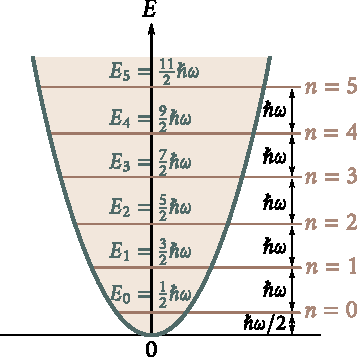
\includegraphics[scale=1]{figures/ch_04/fig_4_3.pdf}
		\caption[]{Energy spectrum of linear harmonic oscillator.}
		\label{fig:4_3}
	\end{center}
	\vspace{-0.7cm}
\end{figure}

The minimum portion of energy that can be absorbed or emitted by the lattice in the process of thermal vibrations corresponds to the transition of the normal mode being excited from the given energy level to the adjacent level and is equal to
\begin{equation}\label{eq:4_16}
    \ab{\varepsilon}{ph} = \hslash \omega.
\end{equation}

\noindent
This portion, or quantum, of energy of thermal vibrations of the lattice is termed a \textit{phonon}.

The following analogy may help to clear up the point. The space inside a black body is filled with equilibrium thermal radiation. From the quantum mechanical point of view such radiation is treated as a gas made up of the light quanta, or photons, whose energy is $\varepsilon= \hslash\omega=h\nu$ and whose momentum is $p=\hslash\omega/c=h/\lambda$, where $c$ is the velocity of light, and $\lambda$ its wavelength.

The field of elastic waves in the crystal may be treated similarly as a gas made up of quanta of the normal modes of the lattice, or of phonons having the energy $\ab{\varepsilon}{ph}=\hslash\omega=h\nu$ and momentum
\begin{equation}\label{eq:4_17}
    \ab{p}{ph} = \frac{\hslash \omega}{v} = \frac{h}{\lambda} = \hslash q
\end{equation}

\noindent
where $v$ is the velocity of sound, and $\lambda$ the length of the elastic wave.

From this point of view a heated crystal may be likened to a box filled with phonon gas. The analogy may be extended.

Phonons are described by the same Bose-Einstein distribution function \eqref{eq:3_54} as photons:
\begin{equation*}
    f(E) = \frac{1}{e^{\ab{\varepsilon}{ph}/(\ab{k}{B}T)} - 1} = \frac{1}{e^{(\hslash\omega)/(\ab{k}{B}T)} - 1}.
\end{equation*}

\noindent
Depending on the intensity of excitation of the normal mode it can ``emit'' a definite number of phonons. Thus, if some normal mode was excited to the third level (\fig{4_3}), its energy became $E_3=(3+1/2)\hslash\omega$; this means that the particular normal mode has ``generated'' three identical phonons each with an energy of $\hslash\omega$.

\begin{figure}[t]
	\begin{center}
		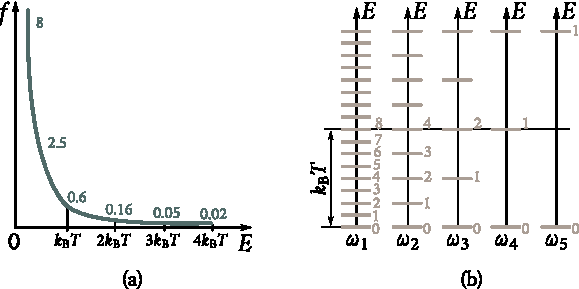
\includegraphics[scale=1]{figures/ch_04/fig_4_4.pdf}
		\caption[]{Energy spectrum of linear harmonic oscillator.}
		\label{fig:4_4}
	\end{center}
	\vspace{-0.7cm}
\end{figure}

Figure \ref{fig:4_4}(a) shows the graph of the phonon energy (frequency) distribution function $f(E)$. We see that for a given temperature $T$, all normal modes in a lattice up to those with the energy $\hslash\omega\approx\ab{k}{B}T$ are excited; practically no quanta of higher frequencies with the energy $\hslash\omega>\ab{k}{B}T$ are excited. This is quite evident from \fig{4_4}(b).
Horizontal strokes here denote energy spectra of normal modes with the frequencies $\omega_1=\ab{k}{B}T/(8\hslash)$, $\omega_2=\ab{k}{B}T/(4\hslash)$, $\omega_3=\ab{k}{B}T/(2\hslash)$, $\omega_4=\ab{k}{B}T/\hslash$ and $\omega_5=2\ab{k}{B}T/\hslash$; the level corresponding to $\ab{k}{B}T$ is shown by a dotted line.
It follows that for a given temperature $T$ the mode with the frequency $\omega_1$ is excited approximately to the $8$th level. As was stated before, this means that this normal mode ``generates'' eight identical phonons with the energy $\hslash\omega_1=\ab{k}{B}T$ each. The normal mode with the frequency $\omega_2$ is excited approximately to the $4$th level, that with the frequency $\omega_3$ to the
second, and that with the frequency $\omega_4$ (whose quantum of energy is $\hslash\omega_4=\ab{k}{B}T$) to the first. At the same time, the vibration $\omega_5$ is rarely
excited at $T$ because its excitation energy $\hslash\omega_5$ is too high. The excitation of still higher frequencies is a much more rare event. Therefore, we can say that approximately only the vibrations with frequencies not greater than $\omega$ corresponding to the energy $\hslash\omega\approx\ab{k}{B}T$ are excited in a solid at temperatures $T<\Theta$.

By definition, the distribution function $f(E)$ expresses the average number of phonons having the energy $\ab{\varepsilon}{ph}=\hslash\omega$. Therefore, to obtain the average energy of an excited normal mode, $\ab{\overline{E}}{n.m}$, of the frequency $\omega$ one has to multiply \eqref{eq:3_54} by $\hslash\omega$:
\begin{equation}\label{eq:4_18}
    \ab{\overline{E}}{n.m} = \frac{\hslash\omega}{e^{(\hslash\omega)/(\ab{k}{B}T)} - 1}.
\end{equation}

\section{Heat capacity of solids}\label{sec:33}

The thermal energy of a solid $\ab{E}{lattice}$ is the sum of the energies of its normal modes. The number of normal modes per spectral interval $\deriv{\omega}$ is $g(\omega)\,\deriv{\omega}$ [see \eqn{4_8}]. Multiplying this number by the average energy $\ab{\overline{E}}{n.m}$ of the normal mode, \eqref{eq:4_18}, we obtain the total energy of the normal modes in the interval $\deriv{\omega}$
\begin{equation*}
    \deriv{\ab{E}{lattice}} = \ab{\overline{E}}{n.m} g(\omega)\, \deriv{\omega}.
\end{equation*}

\noindent
Integrating this expression over the entire spectrum of the normal modes, that is, from $0$ to $\ab{\omega}{D}$, we obtain the energy of the thermal vibrations of the lattice of a solid:
\vspace{-12pt}
\begin{equation}\label{eq:4_19}
    \ab{E}{lattice} = \int_0^{\ab{\omega}{D}} \ab{\overline{E}}{n.m}\, g(\omega)\, \deriv{\omega}.
\end{equation}

The heat capacity at constant volume of a solid, $C_V$, is the change in the thermal energy of a solid brought about by a one degree change in its temperature. To find it one should differentiate lattice with respect to $T$:
\begin{equation}\label{eq:4_20}
    C_V = \diff{\ab{E}{lattice}}{T}.
\end{equation}

The fundamental problem in the theory of heat capacity is the temperature dependence of $C_V$. Let us first consider it from a qualitative point of view for two temperature ranges: for the range of temperatures much below the Debye temperature
\begin{equation}\label{eq:4_21}
    T \ll \Theta
\end{equation}

\noindent
which is termed the \textit{low temperature range}, and for the range of temperatures above the Debye temperature
\begin{equation}\label{eq:4_22}
    T > \Theta
\end{equation}

\noindent
the term for which is the \textit{high temperature range}.

\textbf{Low temperature range.} In this range mainly the low frequency normal modes, with the energy quanta $\hslash\omega<\ab{k}{B}T$, are excited. The approximate value of the average energy of normal vibrations may in this case be calculated with the aid of the following method. Expand the denominator of expression \eqref{eq:4_18} into a series leaving only two terms:
\begin{equation*}
    \ab{\overline{E}}{n.m} = \frac{\hslash\omega}{e^{(\hslash\omega)/(\ab{k}{B}T)} - 1} \approx \frac{\hslash\omega}{1 + \dfrac{\hslash\omega}{\ab{k}{B}T} + \ldots - 1} \approx \ab{k}{B}T.
\end{equation*}

\noindent
Hence, in the low temperature range the average energy of every normal mode increases in proportion to the absolute temperature $T$:
\begin{equation}\label{eq:4_23}
    \ab{\overline{E}}{n.m} \propto T.
\end{equation}

\noindent
This law is due to the increase in the probability of excitation of every normal mode with the rise in temperature resulting in an increase in its average energy.

In addition to this, the rise in temperature in the low temperature range, causes new higher frequency normal modes to be excited. The approximate number of the latter, $z$, may be calculated with the aid of \eqn{4_8}. If we assume that at a temperature $T$ all normal modes up to the frequency $\omega\approx\ab{k}{B}T/\hslash$ are excited, we get
\begin{equation*}
    z = \int_0^{\ab{k}{B}T/\hslash} g(\omega)\, \deriv{\omega} \approx \int_0^{\ab{k}{B}T/\hslash} \omega^2\, \deriv{\omega} \propto T^3.
\end{equation*}

It follows that with the rise in temperature the number of normal modes increases in proportion to the cube of the absolute temperature:
\begin{equation}\label{eq:4_24}
    z \propto T^3.
\end{equation}

To sum up, the crystal's energy in the low temperature range increases with the rise in temperature by means of two mechanisms: (1) the increase in the average energy of every normal mode, $\ab{\overline{E}}{n.m}$, due to the rise in the probability of its excitation, and (2) the increase in the number of the normal modes of the lattice.

The first mechanism is responsible for the increase in energy proportional to $T$ and the second for the one proportional to $T^3$.

Therefore, the total effect is an increase in the energy of the lattice proportional to $T^4$:
\begin{equation}\label{eq:4_25}
    \ab{\overline{E}}{lattice} \propto T^4
\end{equation}

\noindent
and a rise in heat capacity proportional to $T^3$:
\begin{equation}\label{eq:4_26}
    C_V \propto T^3.
\end{equation}

Formula \eqref{eq:4_26} is the \textit{Debye $T^3$ law}, which agrees well with experiment in the low temperature range.

\textbf{High temperature range.} As has been already stated, all normal modes of a lattice are excited at the Debye temperature, so that a further rise in temperature cannot increase their number. Therefore, the variation in energy of a solid in the high temperature range may only be due to the rise in intensity of the normal modes, resulting in an increase in their average energy $\ab{\overline{E}}{n.m}$. Since $\ab{\overline{E}}{n.m}\propto T$, the variation of the energy of the body as a whole, too, should be proportional to $T$:
\begin{equation}\label{eq:4_27}
    \ab{\overline{E}}{lattice} \propto T
\end{equation}

\noindent
and the heat capacity must be independent of $T$:
\begin{equation}\label{eq:4_28}
    C_V = \diff{\ab{\overline{E}}{lattice}}{T} = \text{constant}.
\end{equation}

Relation \eqref{eq:4_28} is the expression of the \textit{Dulong and Petit law}, which is quite well substantiated by experiment.

A rather wide range of temperatures, the so-called \textit{medium temperature range}, lies between the high and low temperature ranges. In this medium temperature range, gradual transition from the Debye $T^3$ law to the Dulong and Petit law takes place. Calculations in this range are the most difficult.

To sum up, the following physical picture of the variation of the temperature dependence of energy and of heat capacity of a solid with the rise in temperature may be presented.

In the low temperature range ($T\ll\Theta$) the solid's energy increases with the rise in temperature firstly because of the increase in the probability of excitation of every normal mode, that is because of the increase in its average energy, $\ab{\overline{E}}{n.m}$, which is proportional to $T$, and secondly because new normal modes are drawn into the process causing the body's energy to increase in proportion to $T^3$. The energy of the lattice, as a whole, rises in proportion to $T^4$ and the specific heat in proportion to $T^3$.

As the temperature approaches the Debye temperature the second mechanism gradually becomes inoperative and $\ab{E}{lattice}$ becomes less dependent on $T$, causing a deviation from the Debye $T^3$ law.

At the Debye temperature, the entire spectrum of normal modes is excited. Therefore, the second mechanism has no part to play; only the first mechanism operates here causing the energy to rise in proportion to $T$ and the heat capacity $C_V$ to remain independent of $T$ (the Dulong and Petit law).

The qualitative laws of the variation of $C_V$ with $T$ obtained from the study of physical processes in solids may be substantiated by more rigorous quantitative calculations. To this end let us turn to \eqref{eq:4_19} and try to calculate the lattice energy as a function of temperature more accurately.

Substituting $g(\omega)$ from \eqn{4_14}, and $\ab{\overline{E}}{n.m}$ from \eqref{eq:4_18} into \eqref{eq:4_19}, we obtain
\begin{equation}\label{eq:4_29}
    \ab{E}{lattice} = \frac{9N}{\ab{\omega}{D}^3} \int_0^{\ab{\omega}{D}} \frac{(\hslash\omega)^3}{e^{(\hslash\omega)/(\ab{k}{B}T)} - 1}\, \deriv{\omega}.
\end{equation}

One can introduce the dimensionless quantity $x=(\hslash\omega)/(\ab{k}{B}T)$ and rewrite \eqref{eq:4_29} in the form
\begin{equation}\label{eq:4_30}
    \ab{E}{lattice} = 9N \ab{k}{B} \Theta \parenthesis{\frac{T}{\Theta}}^4 \int_0^{\Theta/T} \frac{x^3}{e^x - 1}\, \deriv{x}
\end{equation}

\noindent
where $\Theta$ is the Debye temperature.

We will consider the high and the low temperature ranges separately.

\textbf{Low temperature range ($T\ll\Theta$)}. In this range we can substitute infinity for the limit of integration in \eqref{eq:4_30}. Taking into account that
\begin{equation*}
    \frac{x^3}{e^x - 1}\, \deriv{x} = \frac{\pi^4}{15}
\end{equation*}

\noindent
we obtain
\begin{equation}\label{eq:4_31}
    \ab{E}{lattice} = \frac{3\pi^4}{5} N \ab{k}{B} \Theta \parenthesis{\frac{T}{\Theta}}^4 \propto T^4.
\end{equation}

\noindent
Differentiating \eqn{4_31} with respect to temperature, we obtain
\begin{equation}\label{eq:4_32}
    C_V = \frac{12\pi^4}{5} N \ab{k}{B} \parenthesis{\frac{T}{\Theta}}^3 \propto T^3.
\end{equation}

\noindent
We have arrived at the Debye $T^3$ law in accordance with which the heat capacity of a lattice varies in the low temperature range as the cube of the temperature.

\textbf{High temperature range.} For such temperatures the values of $x$ are small and, hence, it is possible to drop all but the first two terms of the expansion $e^x=1+x+\ldots$. Then,
\begin{equation}\label{eq:4_33}
    \ab{E}{lattice} = 9N \ab{k}{B} \Theta \parenthesis{\frac{T}{\Theta}}^4 \int_0^{\Theta/T} x^2\, \deriv{x} = 3N \ab{k}{B} T \propto T.
\end{equation}

\noindent
The heat capacity of the crystal is
\begin{equation}\label{eq:4_34}
    C_V = \diff{\ab{E}{lattice}}{T} = 3N \ab{k}{B} = \text{constant}.
\end{equation}

For a mole of a monatomic substance $N=\ab{N}{A}=\SI{6.023e-23}{\per\mole}$ (Avogadro's number), $\ab{N}{A}\ab{k}{B}=R\approx\SI{8.31}{\joule\per\mole\per\kelvin}$ (the gas constant) and
\begin{equation}\label{eq:4_35}
    C_V \approx 3R \approx \SI{25}{\joule\per\mole\per\kelvin}.
\end{equation}

Formula \eqref{eq:4_35} expresses the Dulong and Petit law, which was formulated by them in 1819.

The solid line in \fig{4_5} shows the theoretical temperature dependence of the heat capacity of solids, the points being experimental values for silver, diamond, aluminium, copper, and rock salt. The agreement between theory and experiment is quite satisfactory not only from the qualitative but also from the quantitative point of view.

\begin{figure}[t]
	\begin{center}
		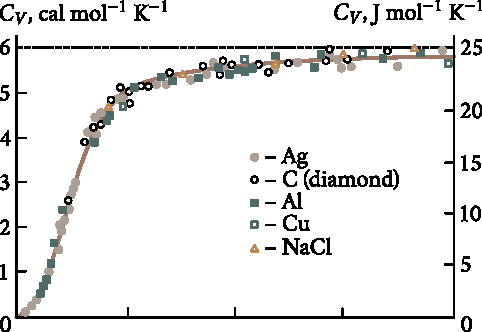
\includegraphics[scale=0.98]{figures/ch_04/fig_4_5.pdf}
		\caption[]{Temperature dependence of heat capacity of solids. The solid line is the theoretical Debye curve.}
		\label{fig:4_5}
	\end{center}
	\vspace{-0.6cm}
\end{figure}

Knowing the temperature dependence of the energy of a lattice, we can easily find at least the qualitative dependence of the concentration of the phonon gas on temperature, that is, the number of phonons $\ab{n}{ph}$ excited in a unit of volume of the crystal.

The concentration of the phonon gas in the low temperature range, in which $\ab{E}{lattice}\propto T^4$ and the phonon energy $\hslash\omega\approx\ab{k}{B}T\propto T$, must be proportional to $T^3$:
\begin{equation}\label{eq:4_36}
    \ab{n}{ph} \propto T^3.\quad \text{(low temperature range, $T\ll\Theta$)}
\end{equation}

In the high temperature range, where $\ab{E}{lattice}\propto T$ and the phonon energy attains the maximum value of $\hslash\ab{\omega}{D}\approx\ab{k}{B}T$ independent of $T$, the concentration of the phonon gas should be proportional to $T$:
\begin{equation}\label{eq:4_37}
    \ab{n}{ph} \propto T.\quad \text{(high temperature range, $T>\Theta$)}
\end{equation}

To be exact, to calculate the concentration of the phonon gas one must know the average energy of the phonons $\ab{\overline{\varepsilon}}{ph}$ both in the low and the high temperature ranges since the lattice energy is equal to the product of the average phonon energy and their concentration. The calculation of $\ab{\overline{\varepsilon}}{ph}$ yields
\begin{equation}\label{eq:4_38}
    \ab{\overline{\varepsilon}}{ph} = \frac{\pi^2\ab{k}{B}T}{5}
\end{equation}

\noindent
for the low temperature range, and
\begin{equation}\label{eq:4_39}
    \ab{\overline{\varepsilon}}{ph} = \frac{2\ab{k}{B}\Theta}{3}
\end{equation}

\noindent
for the high temperature range.

This justifies the temperature dependence of $\ab{n}{ph}$ expressed by formulae \eqref{eq:4_36} and \eqref{eq:4_37} and obtained by qualitative methods.

\section{Heat capacity of electron gas}\label{sec:34}

The metals, in addition to ions, which constitute the lattice and vibrate around their equilibrium positions, contain also free electrons, the number of which per unit volume is approximately the same as that of the ions. For this reason, the specific heat of a metal should be the sum of the heats capacity of the lattice $\ab{C}{lattice}$ calculated in the previous paragraph and of the electron gas $\ab{C}{e}$:
\begin{equation*}
    C_V = \ab{C}{lattice} + \ab{C}{e}.
\end{equation*}

If the electron gas was a normal classical (nondegenerate) gas, every electron would have an average energy $3\ab{k}{B}T/2$ and the energy of the electron gas per mole of the metal would be
\begin{equation*}
    \abc{E}{e}{(cl)} = \frac{3}{2} \ab{N}{A} \ab{k}{B} T = \frac{3}{2} RT
\end{equation*}

\noindent
and its heat capacity would be
\begin{equation}\label{eq:4_40}
    \abc{C}{e}{(cl)} = \frac{3}{2} \ab{N}{A} \ab{k}{B} = \frac{3}{2} R.
\end{equation}

\noindent
The total heat capacity of the metal in the high temperature range would in this case be
\begin{equation*}
    C_V = \ab{C}{lattice} + \ab{C}{e} = \frac{9}{2} R \approx \SI{37}{\joule\per\mole\per\kelvin}.
\end{equation*}

\noindent
Actually, the heat capacity of metals, as well as that of dielectrics, in the high temperature range, where the Dulong and Petit law is valid, is $C_V\approx\SI{25}{\joule\per\mole\per\kelvin}$, a proof that the contribution of the electron gas is negligible.

This situation incomprehensible from the point of view of classical physics found its natural explanation in quantum theory.

Indeed, as was demonstrated in Chapter \ref{chap:3}, the electron gas in metals is a degenerate gas described by the Fermi-Dirac quantum statistics. As the temperature is raised, not all the electrons are thermally excited; only a negligible fraction of them, $\Delta{N}$, occupying states close to the Fermi level (see \fig{3_6}) are thermally excited. The number of such electrons is approximately expressed by the relation \eqref{eq:3_43}:
\begin{equation*}
    \Delta{N} \approx N \frac{\ab{k}{B} T}{2 \ab{E}{F}}
\end{equation*}

\noindent
where $\ab{E}{F}$ is the Fermi energy. For copper at $T\approx\SI{300}{\kelvin}$ and $\ab{E}{F}\approx\SI{7}{\electronvolt}$, we have $\Delta{N}/N\approx 0.002$, that is, less than one percent.

Every thermally excited electron absorbs an energy of the order of $\ab{k}{B}T$ just as a particle of a normal gas does. The energy absorbed by the electron gas as a whole is the product of $\ab{k}{B}T$ and the number of thermally excited electrons $\Delta{N}$:
\begin{equation}\label{eq:4_41}
    \ab{E}{e} \approx \ab{k}{B} T \Delta{N} \approx N \ab{k}{B} T \frac{\ab{k}{B} T}{2 \ab{E}{F}}.
\end{equation}

\noindent
The heat capacity of the electron gas is
\begin{equation}\label{eq:4_42}
    \ab{C}{e} = \diff{\ab{E}{e}}{T} \approx N \ab{k}{B} \frac{\ab{k}{B} T}{\ab{E}{F}}.
\end{equation}

A more accurate calculation yields the following expression:
\begin{equation}\label{eq:4_43}
    \ab{C}{e} \approx \pi^2 N \ab{k}{B} \frac{\ab{k}{B} T}{2 \ab{E}{F}}.
\end{equation}

\noindent
Comparing \eqn{4_40} with \eqref{eq:4_43}, we obtain
\begin{equation}\label{eq:4_44}
    \frac{\ab{C}{e}}{\abc{C}{e}{(cl)}} \approx \pi \frac{\ab{k}{B} T}{\ab{E}{F}}.
\end{equation}

It follows from \eqn{4_44} that the ratio of the heat capacity of a degenerate electron gas to that of a nondegenerate monatomic gas is approximately equal to the ratio of $\ab{k}{B}T$ to $\ab{E}{F}$. At normal temperatures, the ratio $\pi\ab{k}{B}T/\ab{E}{F}\lesssim 1\%$. Therefore,
\begin{equation}\label{eq:4_44p}
    \ab{C}{e} \lesssim 0.01 \abc{C}{e}{(cl)}. \tag{4.44$'$}
\end{equation}

Hence, because of the degeneracy of the electron gas in metals even in the high temperature range only a small portion of the free electrons (usually less than one percent) is thermally excited; the rest do not absorb heat. This is why the heat capacity of the electron gas is negligible as compared to that of the lattice, and the heat capacity of a metal as a whole is practically equal to the latter.

The situation is different in the low temperature range close to absolute zero. Here, the heat capacity decreases in proportion to $T^3$, with the fall in temperature and close to absolute zero may prove to be so small that the contribution of the heat capacity of the electron gas, $\ab{C}{e}$, which decreases much more slowly than $\ab{C}{lattice}$ ($\ab{C}{e}\propto T$), may become predominant. Figure \ref{fig:4_6} shows the temperature dependence of the lattice and electron components of specific heat of an alloy ($20\%$ vanadium and $80\%$ chromium) whose Debye temperature is $\Theta=\SI{500}{\kelvin}$.
It may be seen from \fig{4_6}, that close to absolute zero the heat capacity of the electron gas is much greater than that of the lattice ($\ab{C}{lattice}<\ab{C}{e}$), the sign of the inequality remaining the same up to $T\approx\SI{8.5}{\kelvin}$. At $T>\SI{8.5}{\kelvin}$,
the sign is reversed, the inequality becoming stronger with the rise in $T$. Already at $T\approx\SI{25}{\kelvin}$, the heat capacity of the alloy is mainly due to that of its lattice (at $T=\SI{25}{\kelvin}$ the heat capacity is $\ab{C}{lattice}\approx 10\ab{C}{e}$).

\begin{figure}[t]
	\begin{center}
		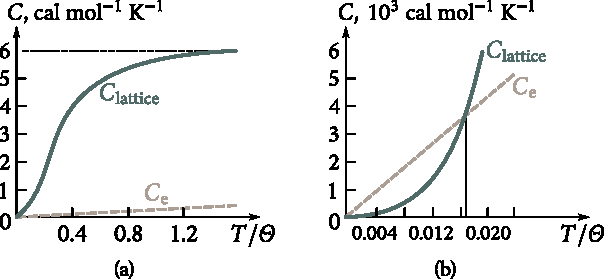
\includegraphics[scale=1]{figures/ch_04/fig_4_6.pdf}
		\caption[]{Temperature dependence of lattice and of an alloy consisting of $20\%$ vanadium and $80\%$ chromium.}
		\label{fig:4_6}
	\end{center}
	\vspace{-0.7cm}
\end{figure}

\section{Thermal expansion of solids}\label{sec:35}

To explain the elastic properties of solids, in Chapter \ref{chap:2} we have introduced the harmonic approximation according to which the elastic force acting on a particle displaced from its equilibrium position is proportional to the displacement [see \eqn{2_3}] and its potential energy is proportional to the square of the displacement [see \eqn{2_2}]; this fact, is represented by a parabola (the dotted line in \fig{2_1}).

The immediate result of the harmonic approximation was the Hooke's law, which describes the elastic deformation of solids. The same approximation was used in Chapter \ref{chap:3} as a basis for calculating the thermal vibrations of a lattice and constructing the theory of heat capacity of a lattice, which is in fair agreement with experiment.

However, the harmonic approximation was unable to explain such well known phenomena as, for instance, the thermal expansion of solids, their heat conductivity, etc.

Indeed, let us turn to the dependence of the potential energy of interaction of the particles of a solid on the distance between them (\fig{4_7}). At absolute zero, the particles occupy positions $r_0$ corresponding to the minimum interaction energy $U_0$ (at the bottom of the potential trough (well) ``abc''). Those distances determine the dimensions of the body at absolute zero. As the temperature rises the particles begin to vibrate around their equilibrium positions $0$. For the sake of simplicity, let us assume that particle $1$ is fixed and only particle $2$ is vibrating. The kinetic energy of the vibrating particle is at its maximum $\ab{E}{k}$ when the particle passes its equilibrium position $0$. In \fig{4_7} the energy $\ab{E}{k}$ is measured upwards from the bottom of the potential trough. When particle $2$ moves to the left, its kinetic energy is used to overcome the repulsive forces acting from particle $1$ and is transformed into the potential energy of the particles' interaction. The displacement to the left stops when all the kinetic energy
$\ab{E}{k}$ is transformed into the potential energy. In the extreme left position of particle $2$ displaced by the distance $x_1$, the potential energy's increment is $U(x_1)=\ab{E}{k}$ and its value $-[U_0-U(x_1)]$. When particle $2$ moves to the right, its kinetic energy is spent to overcome the forces of attraction to particle $1$ and is, as in the previous case, transformed into the potential energy of the particles' interaction. At point B displaced from the equilibrium position by the distance $x_2$, the entire kinetic energy $\ab{E}{k}$ is transformed into the potential energy, the latter increasing by $U(x_2)=\ab{E}{k}$ to become $-[U_0-U(x_2)]$.

\begin{figure}[t]
	\begin{center}
		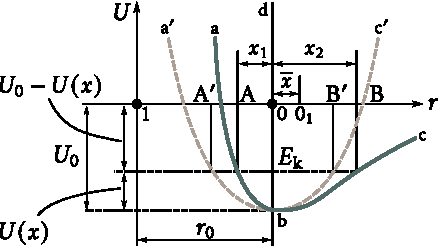
\includegraphics[scale=1]{figures/ch_04/fig_4_7.pdf}
		\caption[]{The origin of thermal expansion of solids (explanation in text).}
		\label{fig:4_7}
	\end{center}
	\vspace{-0.7cm}
\end{figure}

If the vibrations of particle $2$ were purely harmonic, the force $f(x)$ caused by its displacement from the equilibrium position by a distance $x$ would be strictly proportional to this displacement and directed towards the equilibrium position:
\begin{equation}\label{eq:4_45}
    f = - \beta x.
\end{equation}

The change in the particle's potential energy $U(x)$ would, in this case, be described by the parabola a$'$bc$'$ (\fig{4_7}) whose equation is
\begin{equation}\label{eq:4_46}
    U(x) = \frac{\beta x^2}{2}.
\end{equation}

\noindent
This parabola is symmetric about the straight line bd passing parallel to the axis of ordinates at a distance of $r_0$ from it. Therefore, the displacements $x_1$ and $x_2$ would be equal in magnitude and the centre of AB would coincide with the equilibrium position $0$. In this case, heating a body would not bring about its expansion, for a rise in temperature would result only in an increase in the particles' amplitude of vibrations, the average distances between them remaining unchanged.

Actually, the potential curve abc is, as may be seen from \fig{4_7}, not symmetric about the straight line bd, its left branch ba rising much more steeply than the right branch be. This means that the vibrations of the particles in a solid are anharmonic (not harmonic). To account for the asymmetry of the potential curve an additional term
$-gx^3/3$ expressing this asymmetry ($g$ is a proportionality factor) should be introduced. Then, Eqs. \eqref{eq:4_45} and \eqref{eq:4_46} will assume the following form:
\begin{align}
    U(x) &= \frac{\beta x^2}{2} - \frac{g x^3}{3}\tag{4.45$'$},\label{eq:4_45p}\\
    f(x) &= -\diffpartial{U}{x} = -\beta x + g x^2\tag{4.46$'$}.\label{eq:4_46p}
\end{align}

\noindent
When the particle $2$ is displaced to the right ($x>0$), the term $gx^3/3$ is subtracted from $\beta x^2/2$ and the slope of the branch be is less than that of the branch be'; when the displacement is to the left ($x<0$), the term $gx^3/3$ is added to $\beta x^2/2$ and the slope of ba is greater than that of ba'.

Because of the asymmetric nature of the potential curve, the right and left displacements of particle $2$ turn out to be different, the former being greater than the latter (\fig{4_7}). As a result, the central position of particle $2$ (point $0_1$) no longer coincides with its equilibrium position $0$ but is displaced to the right. This corresponds to an increase in the average distance between the particles by $x$.

Hence, heating a body should result in an increase in the average distances between particles and the body should expand. The cause of this is the anharmonic nature of the vibrations of particles making up the solid due to the asymmetry of the dependence of the particles' interaction energy on the distance between them.

Let us estimate the value of the thermal expansion coefficient.

The average value of the force caused by the displacement of particle $2$ from its equilibrium position is
\begin{equation*}
    \overline{f} = -\beta \overline{x} + g \overline{x^2}.
\end{equation*}

\noindent
When the particle vibrates freely, $\overline{f}=0$; therefore, $g\overline{x^2}=\beta\overline{x}$. Hence, we obtain
\begin{equation}\label{eq:4_47}
    \overline{x} = \frac{g\overline{x^2}}{\beta}.
\end{equation}

The expression for the potential energy of a vibrating particle correct to the second order of magnitude is \eqref{eq:4_45} and its average value is $\overline{U}(x)\approx\beta\overline{x^2}/2$. Hence,
\begin{equation*}
    \overline{x^2} \approx \frac{2 \overline{U}(x)}{\beta}.
\end{equation*}

\noindent
Substituting this into \eqn{4_47}, we obtain
\begin{equation*}
    \overline{x} = \frac{2 g \overline{U}(x)}{\beta^2}.
\end{equation*}

In addition to potential energy $U(x)$, a vibrating particle has kinetic energy $\ab{E}{k}$ such that $\overline{U}(x)=\ab{\overline{E}}{k}$. The total average energy of the particle is $\overline{E}=\overline{U}(x)+\ab{\overline{E}}{k}=2\overline{U}(x)$. This fact makes it possible to rewrite the expression for $x$ in the following form:
\begin{equation*}
    \overline{x} = \frac{g \overline{E}}{\beta^2}.
\end{equation*}

\noindent
The relative linear expansion, that is, the ratio of the variation of the average distance between the particles, $x$, to the equilibrium distance between them, $r_0$, is equal to
\begin{equation*}
    \frac{\overline{x}}{r_0} = \frac{g}{\beta^2 r_0} \overline{E}
\end{equation*}

\noindent
and the \textit{linear expansion coefficient} is
\begin{equation}\label{eq:4_48}
    \alpha = \frac{1}{r_0} \diff{\overline{x}}{T} = \frac{g}{\beta^2 r_0} \diff{\overline{E}}{T} = \chi c_V
\end{equation}

\noindent
where
\begin{equation}\label{eq:4_49}
    \chi = \frac{g}{\beta^2 r_0}
\end{equation}

\noindent
and $c_V$ is heat capacity per particle.

Thus, the thermal expansion coefficient proves to be proportional to temperature. Figure \ref{fig:4_8} shows the temperature dependence of $c_V$ and $\alpha$. It can be easily seen that both are interrelated.

\begin{figure}[t]
	\begin{center}
		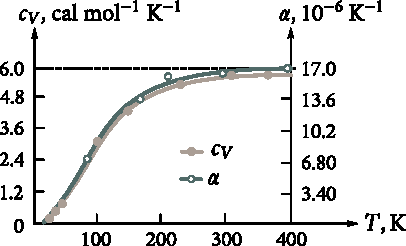
\includegraphics[scale=1]{figures/ch_04/fig_4_8.pdf}
		\caption[]{Temperature dependence of linear expansion coefficient a and of heat capacity $c_V$ of copper.}
		\label{fig:4_8}
	\end{center}
	\vspace{-0.7cm}
\end{figure}

In the high temperature range the energy of a particle engaged in linear vibrations is $\ab{k}{B}T$ and its heat capacity is $c_V=\ab{k}{B}$. Therefore, the thermal expansion coefficient of a linear atomic chain will be
\begin{equation*}
    \alpha = \chi c_V = \frac{g \ab{k}{B}}{\beta^2 r_0}.
\end{equation*}

\noindent
Substituting the values for $g$, $\ab{k}{B}$, $\beta$, and $r_0$ for various solids, we obtain a value of the order of \num{e-4} to \num{e-5} for $\alpha$, which is in fair agreement with experiment. Experiment also supports the conclusion that in the high temperature range $\alpha$ is practically independent of temperature (\fig{4_8}).

In the low temperature range $\alpha$ behaves in a way similar to that of $c_V$: it decreases with the fall in temperature and tends to zero as absolute zero is approached.

In conclusion, we would like to remark that for metals a formula similar to \eqref{eq:4_48} was first proposed by E. Gr\"uneisen in the form
\begin{equation}\label{eq:4_50}
    \alpha = \frac{\gamma \varkappa}{3 V} c_V
\end{equation}

\noindent
where $\varkappa$ is the metal's compressibility, $V$ the atomic volume, and $\gamma$ the Gr\"uneisen constant, ranging from $1.5$ to $2.5$, depending on the metal.

\section{Heat conductivity of solids}\label{sec:36}

\textbf{Heat conductivity of dielectrics (lattice heat conductivity).} The second effect caused by the anharmonic nature of atomic vibrations is the \textit{thermal resistance} of solids. There could be no such resistance should the atomic vibrations be strictly harmonic propagating through the lattice in the form of noninteracting elastic waves. In
the absence of interaction, the waves would be able to travel without scattering, that is, without meeting any resistance, like light in vacuum.

If we were to set up a temperature difference in such a crystal, the atoms of the hot end vibrating with large amplitudes would transmit their energy to the neighbouring atoms and the front of the heat wave would travel along the crystal with the velocity of sound. Because the wave would meet no resistance there would be a considerable heat flux even for an infinitesimally small temperature difference and the heat conductivity of the crystal would be infinitely great.

The nature of atomic vibrations in real crystals at temperatures not too low is anharmonic, as indicated by the second term in \eqn{4_45p}. The anharmonicity destroys the independence of the normal modes of the lattice and causes them to interact, exchanging energy and changing the direction of their propagation (through mutual scattering). It is just those processes of interaction between the elastic waves that make possible the transfer of energy from the modes of one frequency to the modes of another and the establishment of thermal equilibrium in the crystal.

The process of mutual scattering of normal modes is conveniently described in terms of phonons, the thermally excited crystal being regarded as a box containing phonons. In the harmonic approximation, in which the normal modes are presumed to be independent, the phonons make up an ideal gas (a gas of noninteracting phonons). The transition to the anharmonic modes is equivalent to the introduction of an interaction between phonons, which may result in the splitting of a phonon into two or more phonons and in the formation of a phonon from two other phonons. Such processes are termed \textit{phonon-phonon scattering}. Their probability, as is the case of all scattering processes, is characterized by the \textit{effective scattering cross-section} $\ab{\sigma}{ph}$. Should the phonon be, from the point of view of the scattering processes, represented by a sphere of the radius $\ab{r}{ph}$ then, $\ab{\sigma}{ph}=\pi\ab{r}{ph}^2$. The phonon-phonon scattering may take place only if the phonons approach to within a distance at which their effective cross sections begin to overlap. Since the scattering is due to the anharmonicity of the atomic vibrations, numerically described by the coefficient of anharmonicity $g$, it would be natural to assume that the phonon effective cross section radius is proportional to $g$ and $\ab{\sigma}{ph}\propto g^2$.

Knowing the effective scattering cross section $\ab{\sigma}{ph}$, we can calculate the mean free path $\ab{\lambda}{ph}$ of the phonons, that is, the average distance the phonons travel between two consecutive scattering acts. Calculations show that
\begin{equation}\label{eq:4_51}
    \ab{\lambda}{ph} = \frac{1}{\ab{n}{ph} \ab{\sigma}{ph}} \propto \frac{1}{\ab{n}{ph} g^2}
\end{equation}

\noindent
where $\ab{n}{ph}$ is the phonon concentration.

In the kinetic theory of gases it is proved that for gases the \textit{heat conductivity} is
\begin{equation}\label{eq:4_52}
    \mathcal{K} = \frac{\lambda v C_V}{3}
\end{equation}

\noindent
where $\lambda$ is the mean free path of the molecules, $v$ their thermal velocity, and $C_V$ the heat capacity of the gas.

Let us apply this formula to the phonon gas substituting for $C_V$ the specific heat of the crystal (the phonon gas), for $\lambda=\ab{\lambda}{ph}$ the mean free path of the phonons, and for $v$ the velocity of sound (the phonon velocity). We obtain the following expression for the lattice heat conductivity:
\begin{equation}\label{eq:4_53}
    \ab{\mathcal{K}}{lattice} = \frac{v \ab{\lambda}{ph} C_V}{3}.
\end{equation}

\noindent
Substituting $\ab{\lambda}{ph}$ into \eqref{eq:4_53} from \eqref{eq:4_51}, we obtain
\begin{equation}\label{eq:4_54}
    \ab{\mathcal{K}}{lattice} \propto \frac{v C_V}{\ab{n}{ph} g^2}.
\end{equation}

In the high temperature range, in accordance with \eqref{eq:4_37}, $\ab{n}{ph}\propto T$; hence,
\begin{equation}\label{eq:4_55}
    \ab{\mathcal{K}}{lattice} \propto \frac{v C_V}{T g^2}.
\end{equation}

Since $C_V$ in this range is practically independent of $T$, the lattice thermal conductivity should be inversely proportional to the absolute temperature, which is in qualitative agreement with experiment. Equation \eqref{eq:4_55} also includes the anharmonicity factor $g$ and the sound velocity $v$, which depend substantially on the rigidity of the bonds between the particles of the solid. Bonds of lesser rigidity correspond to lower $v$'s and to greater $g$'s, since the weakening of the bonds makes for greater thermal vibration amplitudes (for a specified temperature) and for greater anharmonicity. Both those factors should, according to \eqref{eq:4_55}, bring about a reduction in $\ab{\mathcal{K}}{lattice}$. This conclusion is supported by experiment. Table \ref{table:4_2} presents the values of sublimation heat $\ab{Q}{s}$, which is a measure of bonding energy, and of the lattice heat conductivity lattice for some covalent crystals with the diamond lattice: diamond, silicon, and germanium.

\begin{table}[!b]
	\renewcommand{\arraystretch}{1.2}
	\caption{}
	\vspace{-0.6cm}
	\label{table:4_2}
	\begin{center}\resizebox{0.7\linewidth}{!}{
			\begin{tabular}{lcc}
				\toprule[1pt]
				\textbf{Substance} & $\ab{Q}{s}, \parenthesis{\SI{e5}{\joule\per\mole}}$ & $\ab{\mathcal{K}}{lattice}, \parenthesis{\si{\watt\per\metre\per\kelvin}}$\\
                \midrule[0.5pt]\midrule[0.5pt]
                Diamond & $71.23$ & $550.0$\\
                Silicon & $46.09$ & $137.0$\\
                Germanium & $37.00$ & $54.00$\\
				\bottomrule[1pt]
			\end{tabular}
	}\end{center}
\end{table}

We see that the decrease in the bond energy from the value of diamond to that of silicon and, finally, germanium is accompanied by a noticeable decrease in the lattice heat conductivity. A more detailed analysis shows that $\ab{\mathcal{K}}{lattice}$ is also strongly dependent of
the mass $M$ of the particles, being less for greater $M$'s. This, to a large extent, accounts for the fact that the lattice heat conductivity of the lighter elements occupying the upper part of the Mendeleev periodic table (\ce{B}, \ce{C}, \ce{Si}) is of the order of tens or even hundreds of watts per metre per kelvin, the corresponding values for the elements of the middle part of the Mendeleev table being several watts per metre per kelvin, and that for the heavier elements occupying the lower part of the periodic table even to several tenths of a watt per metre per kelvin.

A striking feature is that the lattice heat conductivity of crystals with light particles and rigid bonds may be very high. Thus, at room temperature $\ab{\mathcal{K}}{lattice}$ of diamond is greater than the total heat conductivity of the best heat conductive metal, silver: $\ab{\mathcal{K}}{Ag}=\SI{407}{\watt\per\metre\per\kelvin}$.

At temperatures below the Debye temperature there is a sharp drop in phonon concentration with a fall in temperature leading to a sharp increase in their mean free path, so that at $T\ll\Theta/20$ it becomes comparable with the dimensions of the crystal. Since the crystal surface usually is a poor reflector of phonons, any further decrease in temperature does not lead to an increase in $\ab{\lambda}{ph}$, for the latter is determined by the crystal's dimensions only. The temperature dependence of the lattice heat conductivity within this range of temperatures is determined by the temperature dependence of the heat capacity $\ab{C}{V}$. Since $\ab{C}{V}\propto T^3$ in the low temperature range,
$\ab{\mathcal{K}}{lattice}$ too should be proportional to $T^3$:
\begin{equation}\label{eq:4_56}
    \ab{\mathcal{K}}{lattice} \propto T^3.
\end{equation}

\noindent
This result is also in qualitative agreement with experiment. Figure \ref{fig:4_9} shows the temperature dependence of thermal conductivity of synthetic sapphire. In the low temperature range $\ab{\mathcal{K}}{lattice}$ is
indeed approximately proportional to $T^3$.

\begin{figure}[t]
	\begin{center}
		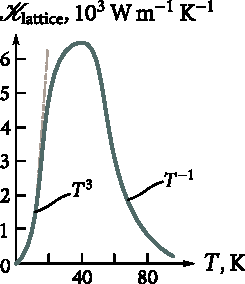
\includegraphics[scale=1]{figures/ch_04/fig_4_9.pdf}
		\caption[]{Temperature dependence of heat conductivity of synthetic sapphire.}
		\label{fig:4_9}
	\end{center}
	\vspace{-0.7cm}
\end{figure}

As the temperature rises so does the concentration of phonons $\ab{n}{ph}$, and this should \textit{per se} cause $\ab{\mathcal{K}}{lattice}$ to rise. However, an increase in $\ab{n}{ph}$ is accompanied by an increase in the phonon-phonon scattering and a consequent decrease in the mean free path of phonons $\ab{\lambda}{ph}$, which should result in a decrease in $\ab{\mathcal{K}}{lattice}$. For low $\ab{n}{ph}$, the first factor should be the predominant one and $\ab{\mathcal{K}}{lattice}$ should rise with $T$.
However, starting with a definite concentration $\ab{n}{ph}$, the second factor should assume primary importance and $\ab{\mathcal{K}}{lattice}$ after passing through a maximum should fall with the rise in $T$. This decrease in the high temperature range is approximately of the $1/T$ type.

Amorphous dielectrics in which the size of regions with a regular structure is of the order of interatomic distances should present a similar picture. Phonon scattering on the boundaries of such regions should be the dominant factor at all $T$'s and, therefore, $\ab{\lambda}{ph}$ should be
independent of $T$. Because of that the heat conductivity of such dielectrics should be proportional to $T^3$ in the low temperature range and independent of $T$ in the high temperature range. This is just what is observed in experiment.

However, at present the theory is unable to predict not only the exact values of lattice heat conductivity, $\ab{\mathcal{K}}{lattice}$, but even its order of magnitude.

\textbf{Heat conductivity of metals.} In metals, in contrast to dielectrics, heat is transported not only by phonons but by electrons as well. Therefore, generally the heat conductivity of metals is the sum of the lattice heat conductivity $\ab{\mathcal{K}}{lattice}$ (conductivity due to phonons) and the heat conductivity $\ab{\mathcal{K}}{e}$ of the free electrons:
\begin{equation*}
    \mathcal{K} = \ab{\mathcal{K}}{lattice} + \ab{\mathcal{K}}{e}.
\end{equation*}

The heat conductivity of the electron gas, can be calculated with the aid of \eqn{4_52}. Substituting into this formula the heat capacity of the electron gas, $\ab{C}{e}$, the electron velocity, $\ab{v}{F}$, and their mean free path, $\ab{\lambda}{e}$, we obtain
\begin{equation}\label{eq:4_57}
    \ab{\mathcal{K}}{e} = \frac{1}{3} \ab{C}{e} \ab{v}{F} \ab{\lambda}{e}.
\end{equation}

\noindent
Substituting $\ab{C}{e}$ from \eqn{4_43} into \eqn{4_57}, we have
\begin{equation}\label{eq:4_58}
    \ab{\mathcal{K}}{e} = \frac{\pi^2}{3} \frac{N \ab{k}{B}^2}{\ab{m}{n} \ab{v}{F}} \ab{\lambda}{e} T.
\end{equation}

Let us make a qualitative estimate of the temperature dependence of heat conductivity of pure metals.

\textbf{High temperature range.} Practically, of all the quantities contained in the right-hand side of \eqn{4_58}, only $\ab{\lambda}{e}$ depends on $T$. For pure metals at temperatures not too low, $\ab{\lambda}{e}$ is determined by electron-phonon scattering and, all other conditions being equal, is inversely proportional to phonon concentration: $\ab{\lambda}{e}\propto 1/\ab{n}{ph}$. In the high temperature range, according to \eqn{4_37}, $\ab{n}{ph}\propto T$. Substituting this into \eqn{4_58}, we obtain
\begin{equation}\label{eq:4_59}
    \ab{\mathcal{K}}{e} = \text{constant}.
\end{equation}

\noindent
Hence, the heat conductivity of pure metals in the high temperature range should be independent of temperature. This is an experimental fact. Figure \ref{fig:4_10} shows the experimental curve depicting the temperature dependence $\mathcal{K}$ for copper. It follows that above $80$-$100$~K the heat conductivity of copper is practically independent of temperature.

\begin{figure}[t]
	\begin{center}
		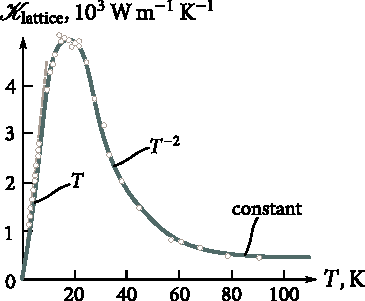
\includegraphics[scale=1]{figures/ch_04/fig_4_10.pdf}
		\caption[]{Temperature dependence of heat conductivity of copper.}
		\label{fig:4_10}
	\end{center}
	\vspace{-0.7cm}
\end{figure}

\textbf{Low temperature range.} The phonon concentration in this range is $\ab{n}{ph}\propto T$, therefore, $\ab{\lambda}{e}\propto 1/T^3$. Substituting into \eqn{4_58}, we obtain
\begin{equation}\label{eq:4_60}
    \ab{\mathcal{K}}{e} \propto T^{-2}.
\end{equation}

Consequently, in the low temperature range where the Debye $T^3$ law is true, the heat conductivity of metals should be inversely proportional to the square of the absolute temperature. This conclusion too is in general supported by experiment (\fig{4_10}).

\textbf{Very low temperature range.} Close to absolute zero the phonon concentration in a metal becomes so small that the main part in electron scattering processes is taken over by the impurity atoms, which are always present in a metal no matter how pure it is. In this case, the mean free path of an electron, $\ab{\lambda}{e}\propto 1/\ab{N}{i}$ ($\ab{N}{i}$, is the concentration of impurity atoms), is no longer dependent on temperature and the heat conductivity of a metal becomes proportional to $T$:
\begin{equation}\label{eq:4_61}
    \ab{\mathcal{K}}{e} \propto T
\end{equation}

\noindent
which is an experimental fact.

Let us estimate the magnitude of $\ab{\mathcal{K}}{e}$ for metals, making use of \eqn{4_57}. For typical metals, we have $\ab{C}{e}\approx 0.01C_V\approx\SI{3e4}{\joule\per\metre\cubed\per\kelvin}$,
$\ab{v}{F}\approx\SI{e6}{\metre\per\second}$, and $\ab{\lambda}{e}\approx\SI{e-8}{\metre}$. Substituting into \eqn{4_57}, we obtain $\ab{\mathcal{K}}{e}\approx\SI{e2}{\watt\per\metre\per\kelvin}$.
Thus, $\ab{\mathcal{K}}{e}$ for metals may be as high as hundreds of watts per metre per kelvin. This is substantiated by experiment. Table \ref{table:4_3} shows the room temperature heat conductivities for some typical metals and for one alloy, constantan, which consists of $60\%$ copper and $40\%$ nickel.

\begin{table}[!b]
	\renewcommand{\arraystretch}{1.2}
	\caption{}
	\vspace{-0.6cm}
	\label{table:4_3}
	\begin{center}\resizebox{0.75\linewidth}{!}{
			\begin{tabular}{lclc}
				\toprule[1pt]
				\textbf{Metal} & $\mathcal{K}, \parenthesis{\si{\watt\per\metre\per\kelvin}}$ & \textbf{Metal} & $\mathcal{K}, \parenthesis{\si{\watt\per\metre\per\kelvin}}$\\
                \midrule[0.5pt]\midrule[0.5pt]
                Silver & $403$ & Aluminium & $210$\\
                Copper & $384$ & Nickel & $60.0$\\
                Gold & $296$ & Constantan & $23.0$\\
				\bottomrule[1pt]
			\end{tabular}
	}\end{center}
\end{table}

It follows that for pure metals $\mathcal{K}$ can indeed be as high as hundreds of watts per metre per kelvin.

Let us also estimate the contribution of the lattice heat conductivity of a metal, making use of Eqs. \eqref{eq:4_53} and \eqref{eq:4_57}:
\begin{equation*}
    \frac{\ab{\mathcal{K}}{lattice}}{\ab{\mathcal{K}}{e}} = \frac{C_V v \ab{\lambda}{ph}}{\ab{C}{e} \ab{v}{F} \ab{\lambda}{e}}
\end{equation*}

\noindent
$v$ being the phonon (sound) velocity. For pure metals, we have $\ab{C}{e}/C_V\approx 0.01$, $v=\SI{5e3}{\metre\per\second}$, $\ab{\lambda}{ph}\approx\SI{e-9}{metre}$, $\ab{v}{F}\approx\SI{e6}{\metre\per\second}$, and $\ab{\lambda}{e}\approx\SI{e-8}{\metre}$.
Hence, $\ab{\mathcal{K}}{lattice}/\ab{\mathcal{K}}{e}\approx\num{5e-2}$.

It follows then that the heat conductivity of typical metals is almost entirely due to the heat conductivity of their electron gas, the contribution of lattice heat conductivity being a few percent. This picture may, however, totally change when we go over to metallic alloys, in which impurity scattering is the principal electron scattering mechanism. The electron mean free path for which such scattering is responsible, $\ab{\lambda}{e}$, is inversely proportional to the impurity concentration $\ab{N}{i}$ ($\ab{\lambda}{e}\propto 1/\ab{N}{i}$) and for high $\ab{N}{i}$'s may become comparable with the phonon mean free path ($\ab{\lambda}{ph}\propto\ab{\lambda}{e}$). Naturally, in such a case the electron contribution to heat conductivity may become of the same order of magnitude as that of the phonon contribution: $\ab{\mathcal{K}}{e}\approx\ab{\mathcal{K}}{lattice}$.
This too is supported by experiment. Table \ref{table:4_3} gives the heat conductivity of constantan. It is much less than that of nickel or copper. This proves the fact that electron scattering in constantan is mainly due to lattice defects caused by impurity atoms. We also note that $\ab{\mathcal{K}}{e}$ and $\ab{\mathcal{K}}{lattice}$ measured by R. Berman in constantan proved to be of the same order of magnitude.

% \begin{figure}[t]
% 	\begin{minipage}[t]{0.52\linewidth}
% 		\begin{center}
% 			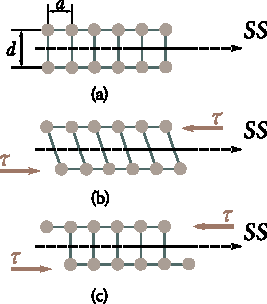
\includegraphics[scale=1]{figures/ch_02/fig_2_7.pdf}
% 			\caption[]{Diagram of rigid shear: (a) --- equilibrium position of atoms in atomic planes adjoining the slip plane; (b) --- gradual shift of one plane in relation to another caused by external stress $\tau$; (c) --- lower atomic plane as a whole displaced by one interatomic distance in relation to the upper plane.}
% 			\label{fig:2_7}
% 		\end{center}
% 	\end{minipage}
% 	\hfill{ }%\hspace{-0.1cm}
% 	\begin{minipage}[t]{0.43\linewidth}
% 		\begin{center}
% 			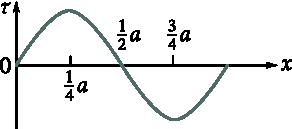
\includegraphics[scale=1]{figures/ch_02/fig_2_8.pdf}
% 			\caption[]{Variation of resistance to shear in the process of displacement of one part of the lattice in relation to another.}
% 			\label{fig:2_8}
% 		\end{center}
% 	\end{minipage}
% \vspace{-0.3cm}
% \end{figure}
